\documentclass[resume]{subfiles}


\begin{document}
\section{Kernel}
\subsection{Compilation}
On configure avec \verb!make linux-menuconfig! (ou \verb!make linux-xconfig!) puis on lance une compilation avec \verb!make linux-rebuild!
\subsubsection{Amélioration}
Comme pour u-boot, on peut utiliser \verb!-fstack-protector-all! pour ajouter une protection sur le stack.\\
Dans le menu, cela se traduit par l'activation de "Strong Stack Protector" et "Stack Protector buffer overflow protection".\\
Le "Randomize va space" permet de placer les éléments à des emplacements mémoire aléatoires (pour éviter d'en cibler un facilement).\\
Il est également possible d'optimiser le kernel pour la place OU pour les performances.\\
Il faut absolument strip avant de déployer (il existe une option pour strip le linux dans le menuconfig).\\
On peut également restreindre l'accès au syslog (system logs).\\
La mise à 0 lors de l'allocation et/ou free de mémoire permet aussi d'éviter certaines attaques
\subsection{Busybox}
Busybox est un éxécutable qui combine beaucoup de fonctions de base (ls, mv, rm, cat, etc...). En mettant toutes ces commandes dans un seul programme, on réduit énormément les redondances et par conséquent la taille de l'éxécutable.\\
On peut également configurer busybox avec \verb!make busybox-menuconfig! puis le compiler avec \verb!make busybox-rebuild!
\subsection{File systems}
Les filesystems doivent être activés dans la configuration de Linux afin d'être utilisables
\subsection{Réseau}
Si le système n'est pas un routeur, on peut choisir de désactiver le routage et le \verb!rp_filter! doit être activé sur toutes les interfaces.
\subsection{Outils}
\begin{itemize}
\item Générateurs de nombres aléatoires
\end{itemize}
\subsection{Attaques}
\begin{center}
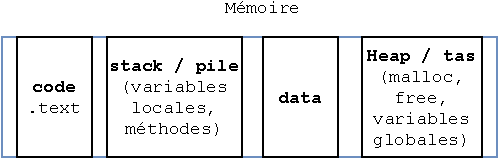
\includegraphics[width=0.6\columnwidth,page=1]{Schemas-crop.pdf}
\end{center}
\paragraph{Éxecution sur le stack} : Ii le stack est éxécutable, il est possible d'y placer du code puis de l'éxécuter (ce qui est de moins en moins le cas).
\paragraph{ret2libc} : Permet de bypasser la non-éxécution du stack. Consiste à éxécuter du code dans une librairie comme libc.
\paragraph{ROP} : Return-Oriented Programming. Éxécution de code malveillant à l'intérieur du programme lui-même
\subsection{Protections}
\label{sec_protections}
\paragraph{ASLR} : Address Space Layout Randomization (changement des adresses de stack et heap) afin d'éviter les attaques \verb!ret2libc!
\paragraph{PIE} : Position de l'éxécutable modifiée pour éviter qu'une attaque soit faite (ou la rendre plus difficile)
\paragraph{Canary} : Variable qui permet de détecter un dépassement dans le stack
\end{document}